%        File: report.tex
%     Created: Sat Nov 03 06:00 PM 2018 E
% Last Change: Sat Nov 03 06:00 PM 2018 E
%
\documentclass[a4paper]{article}
\usepackage{amsmath}
\usepackage{graphicx}
\usepackage{hyperref}
\usepackage[noabbrev,capitalise]{cleveref}
\usepackage{natbib}

\begin{document}

\title{Baby Name Popularity}
\author{
Francisco Rivera \\ \texttt{frivera@college.harvard.edu}
\and
Mark Chamberlain}

\maketitle

\begin{abstract}
The U.S. Census publishes the number of babies born to each first name each year
at the country and state level. These trends exhibit dramatic up- and
down-swings unexplainable by a simple imitation model. We attempt to construct a
model to explain the dynamics of these popularity swings as well as other
stylized facts from the data.
\end{abstract}

\section{The Data}

Our data comes from the U.S.
Census.\footnote{\url{https://catalog.data.gov/dataset/baby-names-from-social-security-card-applications-national-level-data}}
The dataset allows us to observe the number of births in the country each year
by first name and gender with the exception of names for which there were fewer
than five births.

The data requires little processing, but because our aim is to model changes in
popularity rather than population growth, we normalize each data entry as a
percentage of the total number of births that year. To provide a sense of what
some typical trends look like, we plot the popularity of five random
popular\footnote{Defined as exceeding 0.5\% of all births on any year.} names in
\cref{fig:fivenames}.

\begin{figure}[h]
\centering
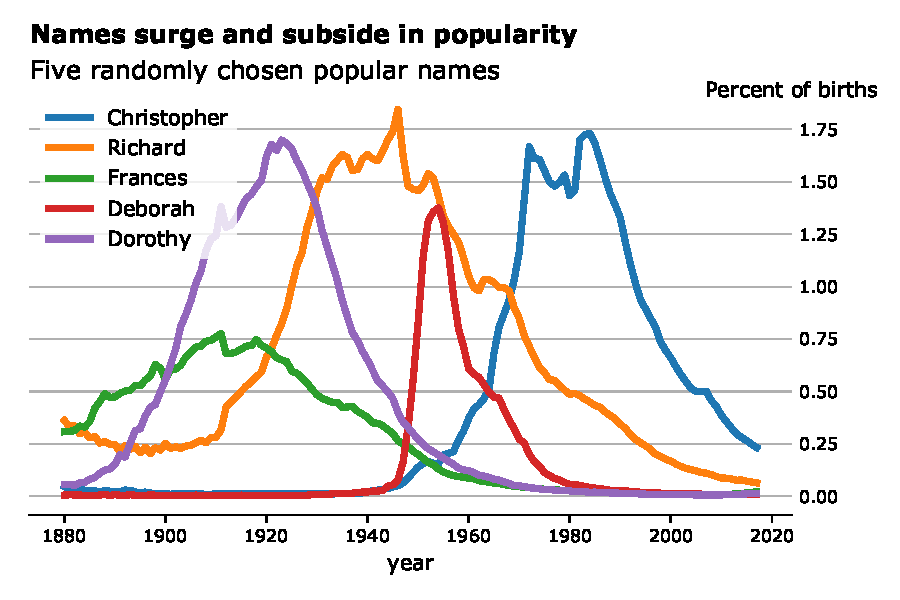
\includegraphics[width=.9\textwidth]{figs/five-rand-names}
\caption{Popularity evolution of five random names}
\label{fig:fivenames}
\end{figure}

On the basis of inspecting many realizations of \cref{fig:fivenames}, for which
the depicted trends are representative, we can take away some stylized facts,

\begin{itemize}
\item The popularity of a name in many cases follows a exponential-like growth
from obscurity, a peak, and then a decay back to obscurity.
\item There appears to be a practical upper-bound to how high the peak is, but
this upper bound need not be binding for many names
\item As ``Deborah'' shows, the down-swing need not be as fast as the up-swing.
\end{itemize}

\section{An Imitation Model}

We will follow \cite{hahn2003drift} closely.

\section{Segmenting the population}

The shortcoming with the imitation model or a model like it is that the
evolution of name popularity appears to behave differently on the up-swing than
the down-swing. This became starkly inconsistent with the imitation model in the
amount of variance we see from year-to-year in name popularity, but even if the
variance matched, we consistently see a boom followed by a bust in name
popularity, which remains unexplainable by this model.

This suggests that there is something different in the adoption of a name at
different points in the stylized lifecycle of popularity. One way to model this
is by segmenting the population, akin to the work on fads done in
\cite{bergman2012fad}. We posit that there are two sub-populations: an ``in''
group and an ``out''-group. ``In''-group membership is desirable, and members of
this group try to distinguish themselves through names distinctive of the group,
but not over-used. However, there is not a separating equilibrium because
members of the out-group also wish to adopt desirable in-group names. Thus, they
too wish to take on names most representative of the in-group. However, we posit
that the out-group will only be able to react to lagged information of name
popularity.

Mathematically, then, in our most general form, we are suggesting if
$p_\text{in}^{(i)}{(t)}$ (respectively $p_\text{out}^{(i)}{(t)}$) are the
proportion of the in-group (respectively out-group) at time $t$ given name $i$,
then our evolution equations are,

\begin{align*}
\frac{d p_\text{in}^{(i)}}{dt} &= \alpha_\text{in} \cdot p_\text{in}^{(i)}
\bigg(K_\text{in} - p_\text{in}^{(i)} - \beta_\text{in} \cdot
p_\text{out}^{(i)}\bigg) \\
\frac{d p_\text{out}^{(i)}(t)}{dt} &= \alpha_\text{out} \cdot p_\text{out}^{(i)}
\bigg( p_\text{in}^{(i)}(t-\tau) - \beta_\text{out} \cdot
p_\text{out}^{(i)}(t-\tau) \bigg)
\end{align*}

In this equations, the $\alpha$ parameters represent a sensitivity of the system
to its pressures, i.e. it calibrates how quickly members of the in and out-group
react to incentives to shift toward or away a name. $K_\text{in}$ represents the
maximal sustainable size of the proportion of the in-group with the name in the
absence of any out-group adopters. The $\beta$ parameters capture aversion to
names being used by members of the out-group, and $\tau$ represents the lag with
which members of the out-group can observe name trends.

\subsection{Numerical simulation}

In order to better understand the behavior these 

\section{Evaluating the model}

\subsection{Qualitative evaluation}

\subsection{Likelihood tests}

\subsection{Pursuing additional data}

\section{Simplifying the model}

\section{Model shortcomings}

\bibliography{sources}
\bibliographystyle{apalike}

\end{document}


